\immediate\write18{makeindex main.nlo -s nomencl.ist -o main.nls}
\documentclass[12pt,oneside]{article}
\usepackage[utf8]{inputenc}
\usepackage[T1]{fontenc}

%----Figures packages
\usepackage{graphicx}
\graphicspath{ {figures/} }
\usepackage{caption}
\usepackage{subcaption}
\usepackage{float}

%----Bibliography  along with 1st line command
\usepackage{nomencl}

%---Math packagesf
\usepackage{amsmath}
\usepackage{amsfonts}
\usepackage{bm}

%---Geometry and style of A4
\usepackage[a4paper,width=150mm,top=25mm,bottom=25mm]{geometry}
\usepackage{fancyhdr}
\pagestyle{fancy}
\renewcommand{\sectionmark}[1]{\markboth{#1}{}} % set the \leftmark
\fancyhf{}

%--Style packages
\renewcommand \thesection{\Roman{section}}
\renewcommand\thesubsection{\Alph{subsection}}
\usepackage{sectsty,textcase}
\subsectionfont{\normalfont\itshape}
\usepackage{titlesec}
\titlelabel{\thetitle.\quad}
\usepackage{titling}


\bibliographystyle{unsrt}

%------Title and Authors
\title{\Huge\textbf{Deep Reinforcement Learning}}
\author{
  Dimitrios Gkouletsos\\
  \texttt{first1.last1@xxxxx.com}
  \and
  Nyquist\\
  \texttt{first2.last2@xxxxx.com}
  \and
  Bode\\
  \texttt{first2.last2@xxxxx.com}
  \and
  Kalman\\
  \texttt{first2.last2@xxxxx.com}
}
\date{\today}

%------------------------BEGIN DOCUMENT-----------------------------------------------------
\begin{document}
\maketitle

%------------------------INTRODUCTION-----------------------------------------------------
\section{Introduction}
	First citation here \cite{sutton} !!!!
	
%------------------------METHODS-----------------------------------------------------
\section{Models and Methods}

%------------------------RESULTS-----------------------------------------------------
\section{Results}
	\begin{figure}[h]
	\centering
	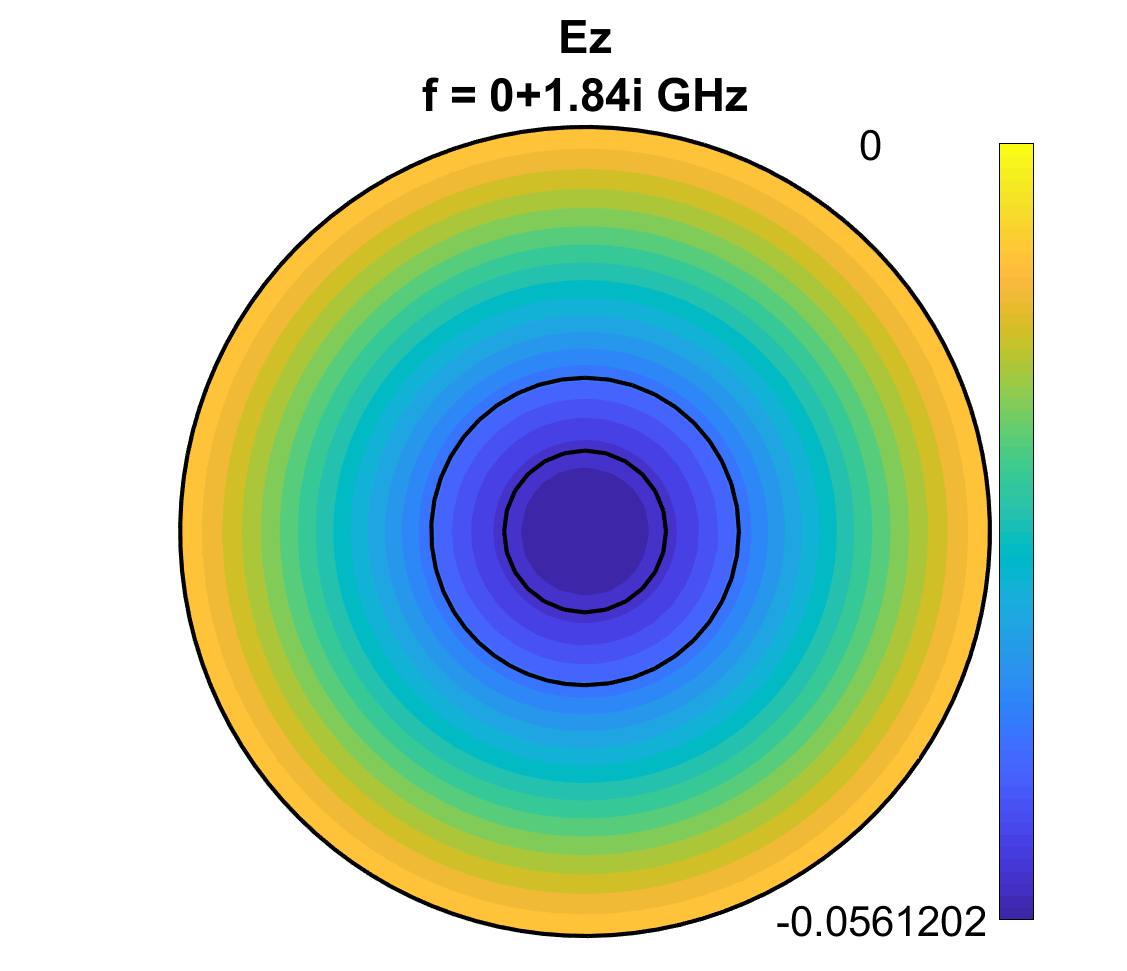
\includegraphics[scale=0.5]{magnitude6}
	\caption{An example graph}
	\label{fig:x cubed graph}
	\end{figure}
	\begin{figure}[h]
     	\centering
     	\begin{subfigure}[b]{0.4\textwidth}
         	\centering
		%trim={<left> <lower> <right> <upper>}
         	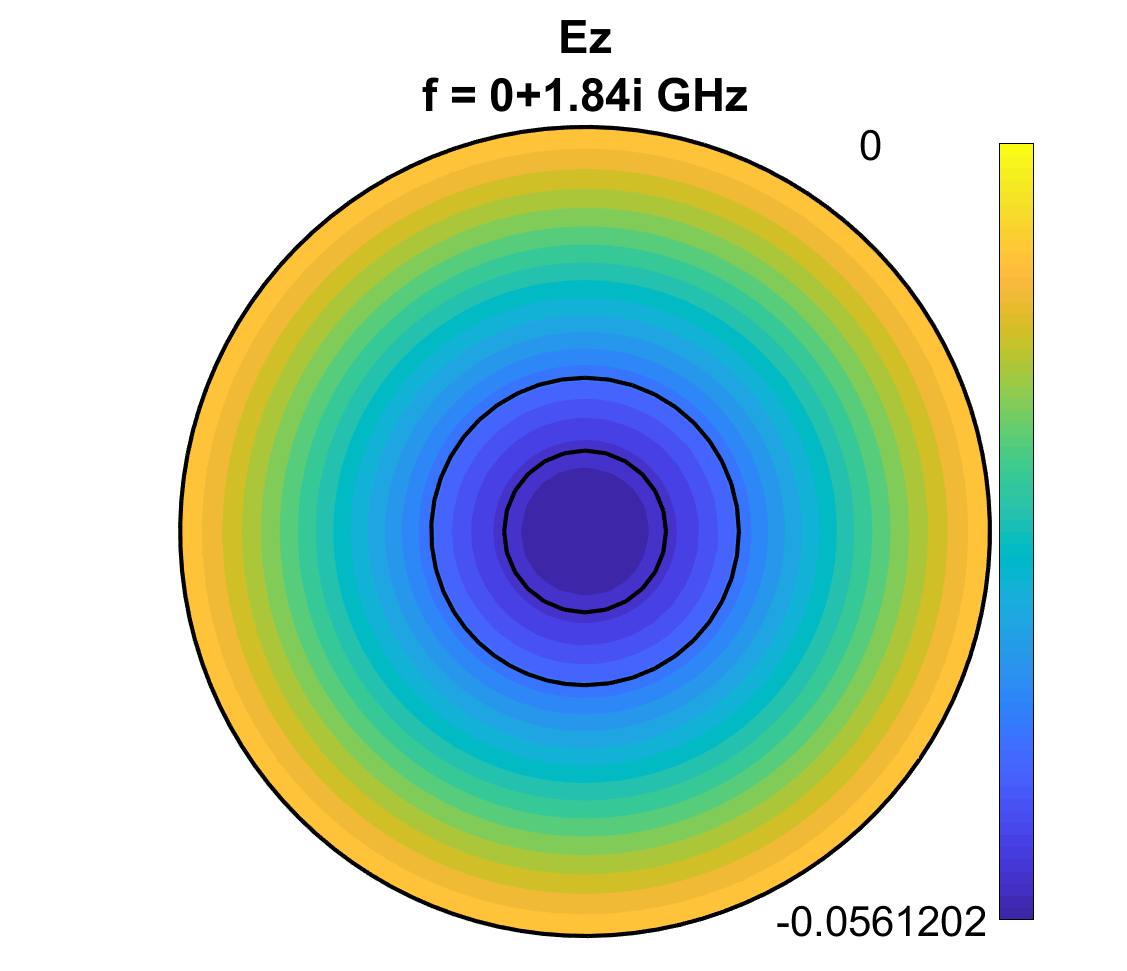
\includegraphics[trim={0cm 0 0cm 0},clip, scale = 0.4]{magnitude6}
         	\caption{$y=x$}
         	\label{fig:y equals x}
     	\end{subfigure}
     	\hfill
     	\begin{subfigure}[b]{0.4\textwidth}
         	\centering
         	\fbox{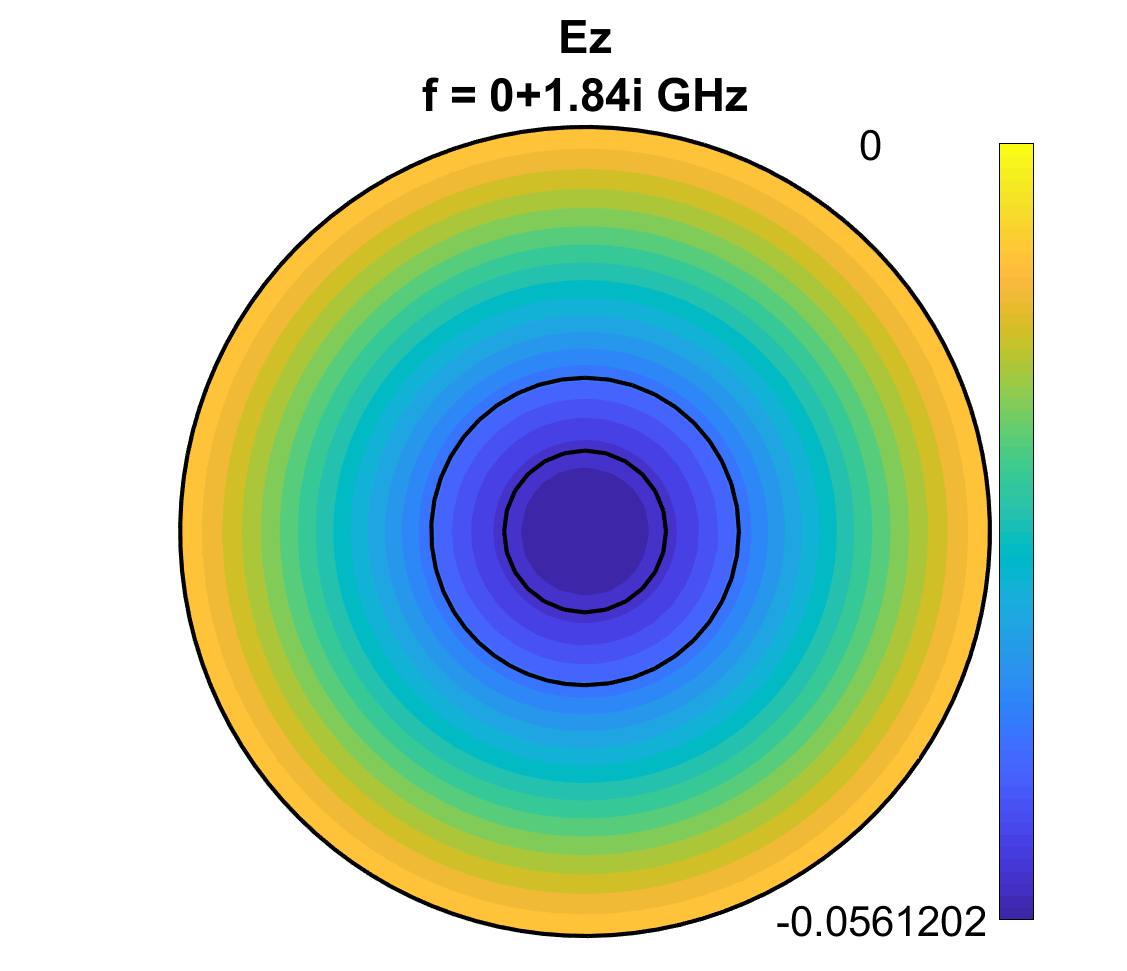
\includegraphics[trim={0cm 0 0cm 0},clip, scale = 0.4]{magnitude6}}
         	\caption{$y=3sinx$}
         	\label{fig:three sin x}
     	\end{subfigure}
     	\caption{Three simple graphs}
     	\label{fig:three graphs}
	\end{figure}
%------------------------DISCUSSION-----------------------------------------------------
\section{Discussion}

%------------------------SUMMARY-----------------------------------------------------
\section{Summary}

%-----------------------REFERENCES----------------------------------------------------
\bibliography{references}

\end{document}